% Clean-view appendix figures: strict-scoring data, with approved figure styles and captions.
\begin{figure*}[!t]

\centering
    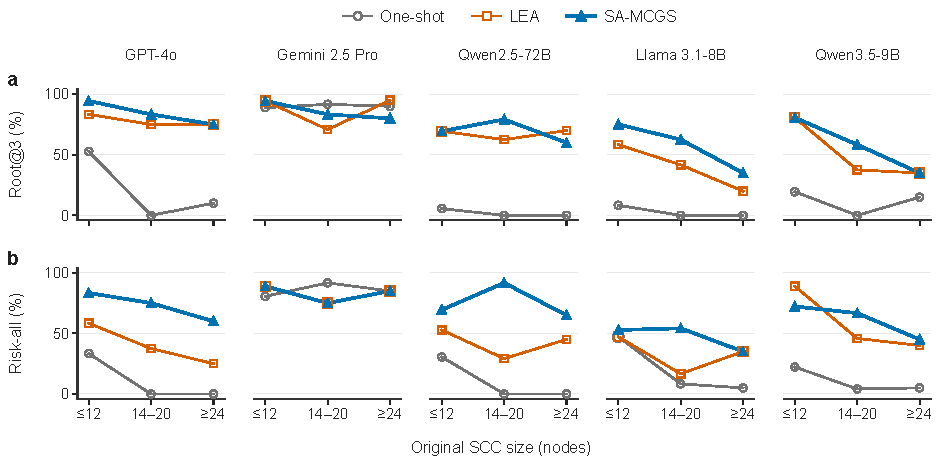
\includegraphics[width=\textwidth]{figures_strict_scoring/fig02_main_results_five_models.pdf}
    \caption{Performance by \scc{} size. Columns correspond to models and rows to (a) \rootthree{} and (b) \riskall{}. All three methods use the same small ($\leq12$ nodes), medium (14--20), and large ($\geq24$) case groups. Gray circles, orange squares, and blue triangles denote One-shot, LEA, and \samcgs{}, respectively.}
    \label{fig:absolute_size_breakdowns}

\end{figure*}

\begin{figure*}[!t]

\centering
    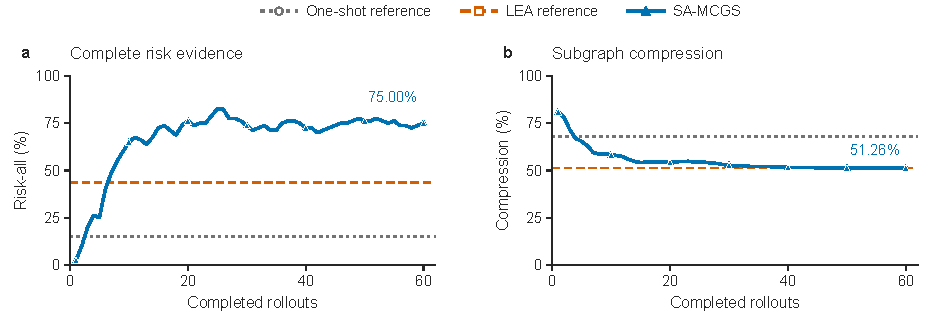
\includegraphics[width=\textwidth]{figures_restored_baseline/fig04_budget_prefix_three_methods.pdf}
    \caption{GPT-4o evidence retention and compression across 60 rollout prefixes on the same 80 cases. The solid curve represents \samcgs{}; horizontal lines indicate the final One-shot and LEA scores. Each prefix is reconstructed from stored search evidence using the final-core selection rule. Results at budget 60 match the final outputs.}
    \label{fig:convergence}

\end{figure*}
